\documentclass[10pt,a4paper]{article}
\usepackage[utf8]{inputenc}
\usepackage{amsmath}
\usepackage{amsfonts}
\usepackage{amssymb}
\usepackage{graphicx}
\usepackage{url}
\usepackage{epstopdf}
\usepackage[ngerman]{babel}
\usepackage[ngerman]{translator}
\usepackage{listings}
\usepackage[singlelinecheck = false]{caption}
\usepackage[colorlinks=true,
        linkcolor=black,
        citecolor=black,
        filecolor=black,
        pagecolor=black,
        urlcolor=black,
        bookmarks=true,
        bookmarksopen=true,
        bookmarksopenlevel=3,
        plainpages=false,
        pdfpagelabels=true]{hyperref}

\parindent 0pt
\pagestyle{headings}

\let\oldsection\section
\renewcommand{\section}{\newpage \oldsection}

\title{
	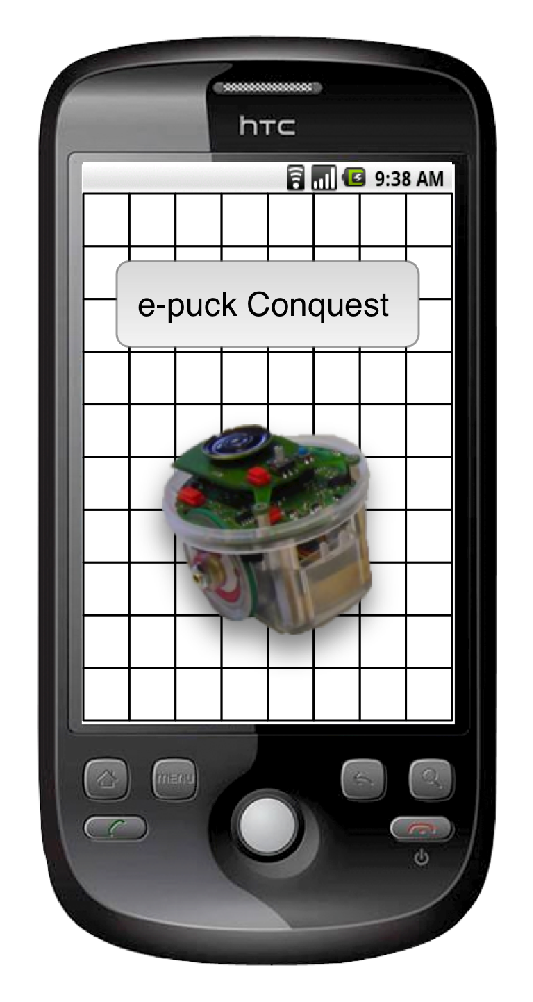
\includegraphics[height=10cm]{images/logo.eps} \\
	\vspace{1cm}
	Benutzerhandbuch \\
	SEP-Conquest
}
\author{Andreas Wilhelm, Andreas Poxrucker, Martin Freund,\\ Max Binder, Florian B\"urchner, Florian Lorenz} 
\begin{document}
\date{14. Januar 2011}
	\maketitle
	\newpage
	\tableofcontents	
	\newpage
\section{Einleitung}
	\subsection{Einf\"uhrung}
		Dieses Projekt richtet sich \"uberwiegend an Forschungsgruppen, Studenten sowie der e-puck Community. Grundlegende Kenntnisse der Programmiersprachen 
		Java und C sowie ein sicherer Umgang mit Compilern werden f\"ur die Verwendung der Software vorausgesetzt. Auch ein geeigneter Umgang mit sensibler 
		Hardware und ein grundlegendes Verst\"andnis f\"ur eingebettete Systeme sind notwendig. Bevor Sie das System zum ersten Mal in Betrieb 
		nehmen, sollten Sie sich  die gesamte Anleitung sorgf\"altig durchlesen, um eine Besch\"adigung der Hardware zu vermeiden. Hierbei m\"ochten wir vor allem auf
		Kapitel \ref{e_puck_bedienung} verweisen, um sich mit dem e-puck Roboter und dessen Bedienung vertraut zu machen. Alle in diesem Handbuch  
		aufgef\"uhrten Programme	sind im Internet zur freien Verf\"ugung gestellt.\\ 
		Das Entwicklerteam \"ubernimmt keinerlei Haftung f\"ur auftretende Probleme oder Sch\"aden. \\ 
	\subsection{Leistungsmerkmale des Systems}
		\begin{itemize}
			\item{Das System unterstützt bis zu sechs e-puck Roboter} \\		
				Es k\"onnen bis zu sechs e-puck Roboter gleichzeitig effizient ein unbekanntes Gebiet erkunden.
			\item{Zwei verschiedene Steuerungsarten} \\
				Das System unterst\"utzt einerseits die Steuerung eines e-puck Roboters durch eine Touch-Steuerung sowie eine Kippsteuerung.
			\item{Kollisionsvermeidung} \\
				Die e-puck Roboter vermeiden Kollisionen mit anderen Teilnehmern.
			\item{Statistikanzeige}
				Durch den Statistik-Dialog und Visualisierungen kann nachvollzogen werden, wie effizient die Roboter erkundet haben.
		\end{itemize}		
\section{Systemanforderungen}
		\subsection{Smartphone mit Android Betriebssystem} 
				Ein bluetoothf\"ahiges Smartphone mit einem Android Betriebssystem ab Version 2.1 und installiertem CyanogenMod ab Version 6.0.1, integrierten 
				Beschleunigungssensoren sowie ein Touch-Display sind erforderlich um das System zu verwenden. Ein Tutorial f\"ur die Installation des Android 
				Betriebssystems inkl. CyanogenMod ist nicht Teil dieses Handbuchs, bitte wenden Sie sich im Problemfall an die Android-Community unter 
				www.android.com
		\subsection{e-puck Roboter ab Hardware Rev. 2} 
				Mindestens ein e-puck Roboter mit Erweiterungsmodul f\"ur Bodensensoren ist zur Erkundung und zum vollst\"andigen Betrieb notwendig.
		\subsection{Computer} 
				Ein Computer mit Bluetoothadapter zum Flashen der e-puck Roboter.
		\subsection{MPLAB ICD 2 oder 3} 
				Zum Ersetzen des Bootloaders auf dem e-puck Roboter wird MPLAB ICD 2 oder 3 inkl. eines Adapterkabels f\"ur den e-puck Roboter ben\"otigt.
\section{Betriebsbedingungen} 
		\subsection{Ausreichende Stromversorgung} 
				Um ein sicheres Ausf\"uren des Gesamtsystems zu gew\"ahrleisten, m\"ussen die Akkus der e-puck Roboter immer vor Inbetriebnahme vollst\"andig
				aufgeladen sein. Ist dies nicht der Fall kann es zu unerwarteten Fehlern kommen und das System zum Absturz bringen!
		\subsection{ Geeignete Bedingungen f\"ur Funknetzwerke} 
				Verwenden Sie die Hardware nicht in der N\"ahe von starken Strahlungsquellen. Dies kann die Bluetoothkommunikation der e-puck Roboter erheblich st\"oren 				und unvorhergesene Fehler erzeugen.
		\subsection{ Gr\"o\ss e des zu erkundenen Terrains} 
				Das Projekt ist darauf ausgelegt ein Feld mit bis zu 500 Knoten zu erkunden. Ist das zu erkundende Spielfeld gr\"o\ss er, reichen die Akku's der e-puck Roboter
				nicht aus, um die Erkundung vollst\"andig durchzuf\"uhren.
		\subsection{ Spielfeldbedinungen} 
				Das Spielfeld besteht ausschlie\ss lich aus gleichgro\ss en quadratischen Feldern, die rasterf\"ormig und zusammenh\"angend angeordnet sind. Ein Feld 
				muss mindestens so gro\ss \ sein, dass ein im Zentrum stehender e-puck Roboter vollst\"andig in das Innere des Feldes passt. Die Erkundung mit den e-puck 
				Robotern ben\"otigt ausreichend reflektierende und innerhalb der Spezifikation liegenden Linien, sowie eine durchgehend gute Beleuchtung des Spielfeldes 
				von oben. Der Untergrund muss eben sein und darf keine rutschige oder teppich\"ahnliche Oberfl\"ache aufweisen, da sich sonst die e-puck Roboter nicht 
				problemlos bewegen k\"onnen. Die e-puck Roboter d\"urfen w\"ahrend der Erkundung nicht ber\"uhrt, verschoben oder vom Spielfeld gehoben werden. Das 
				Spielfeld darf w\"ahrend der Erkundung nicht ver\"andert werden und keine ung\"ultigen Passagen beinhalten. 
		\subsection{ Umgebungsbedinungen} 
				Es d\"urfen nicht mehr als sechs e-puck Roboter und ein Smartphone zur selben Zeit verwendet werden und die Startpositionen der jeweiligen e-puck Roboter
				sind vor Beginn der Erkundung fest zu w\"ahlen.
		\subsection{ Weitere Betriebsbedinungen des Smartphones und der e-puck Roboter} 
				Die weiteren Betriebsbedinungen des Smartphones und der e-puck Roboter k\"onnen den jeweiligen Benutzerhandb\"uchern der Hardware entnommen 
				werden.
\section{Bedienung des e-puck Roboters}
	\label{e_puck_bedienung}

 	\begin{figure}[htbp]
		\begin{minipage}[t]{6.5cm}
			\vspace{0pt}
			\includegraphics[height=6.5cm]{images/puck1.png} 
			\caption{e-puck}
		\end{minipage}
		\hfill
		\begin{minipage}[t]{0.5\textwidth}
			\vspace{5pt}
				\subsection{Power-Switch}
					Zum Ein/Ausschalten des e-puck Roboters.
				\subsection{Selector}
					Der Selector kann auf 16 verschiedene Positionen gebracht werden. Ist der Selector nach Bet\"atigen des Power-Switch auf Position 0, befindet sich der e-
					puck Roboter in der Kalibrierungsphase. In jedem anderen Fall ist der e-puck im Erkundungsmodus.
				\subsection{Power-LED}
					Die Power-LED Leuchtet gr\"un, sobald der e-puck eingeschaltet ist.
		\end{minipage}
   \end{figure}
   
    \begin{figure}[htbp]
		\begin{minipage}[t]{6.5cm}
			\vspace{0pt}
			\includegraphics[height=6.5cm]{images/puck2.png} 
			\caption{Bodensensoren}
			\label{positionierung_epuck}
		\end{minipage}
		\hfill
		\begin{minipage}[t]{0.5\textwidth}
			\vspace{10pt}
				\subsection{Bodensensoren}
						Das Erweiterungsmodul f\"ur die Bodensensoren ist f\"ur dieses Projekt von sehr gro\ss er Bedeutung. Hierbei ist vor allem zu beachten, dass der e-puck 								Roboter	bei der Kalibrierung, sowie beim Erkundungsvorgang immer richtig positioniert ist. Die folgende Abbildung veranschaulicht, wie der Roboter 
						beim Start der Erkundung	stehen muss. Die schwarze Linie muss zwischen den \"au\ss eren Bodensensoren liegen. (siehe Abbildung 				
						\ref{positionierung_epuck})
		\end{minipage}
   \end{figure}
   
\newpage

	\subsection{Kalibrierung}
		Der Kalibrierungsvorgang beginnt damit, dass der Selector des ausgeschalteten e-pucks auf die Position 0 gesetzt wird. Danach muss der Roboter mit allen drei
		Bodensensoren auf eine schwarze Linie gesetzt werden. Nachdem der Roboter mit dem Power-Switch durch den Benutzer aktiviert wurde, f\"ahrt der e-puck ca.
		7 cm nach vorne. Hierbei muss darauf geachtet werden, dass die Fl\"ache vor dem Roboter wei\ss \ ist. Nach erfolgreicher Kalibrierung f\"ahrt der Roboter wieder
		zur\"uck in seine Ausgangsposition. Falls beim Kalibriervorgang ein Fehler aufgetreten ist, blinken die 8 roten LEDs an der Aussenseite des Roboters. 
		Wiederholen Sie dann den Vorgang erneut und achten Sie darauf dass der Roboter richtig positioniert ist. (siehe Abbildung \ref{kalibrierabbildung}) \\
		
		\vspace{30pt}
		 \begin{figure}[htbp]
			\includegraphics[height=8cm]{images/puck3.png} 
			\caption{Kalibriervorgang}
			\label{kalibrierabbildung}
		\end{figure}
\section{Installation}
			\subsection{Vorbereitungen} 
			Vor der Installation und der ersten Inbetriebnahme sind folgende vorbereitenden Schritte notwendig:
			\begin{itemize}
				\item{Die Akku's der e-puck Roboter m\"ussen vollst\"andig geladen sein}
				\item{Download und Installation von MPLAB IDE}
				\item{Download und Installation von PIC30}
				\item{Download und Installation von Tiny-Bootloader}
				\item{Download und Installation der UNIX-Tools f\"ur Windows}
				\item{Download des modifizierten Bootloader f\"ur 16-fache PLL auf dem e-puck Roboter}
			\end{itemize}
			\subsection{Bootloader aufspielen} 
				Wenn alle Vorbereitungen erfolgreich durchge\"uhrt wurden, muss der Bootloader des e-puck Roboters neu geflasht werden. Eine ausf\"uhrliche
				Anleitung hierzu finden Sie unter \\ \url{http://www.gctronic.com/doc/index.php/E-Puck} \\
				Das MPLAB-Projekt, das Sie ben\"otigen wird bei der Software mitgeliefert und befindet sich im Verzeichnis \textit{/trunk/epuck/bootloader/}.
			\subsection{Bluetooth-Verbindung aufbauen} 
				Schalten Sie den e-puck durch Umschalten des Power-Switch ein und starten Sie den \textit{Pairing}-Prozess. Eine ausf\"uhrliche Anleitung finden Sie
				unter  \\ \url{http://www.gctronic.com/doc/index.php/E-Puck} \\
				Nach der Zuweisung eines Com-Ports muss dieser im \textit{TinyBootloader} eingegeben werden.			
			\subsection{Firmware aufspielen} 
				Als letzten Schritt m\"ussen Sie mithilfe des \textit{TinyBootloader} die Firmware auf den e-puck Roboter aufspielen. Ein Manual zu diesem Programm
				ist unter \url{http://www.etc.ugal.ro/cchiculita/software/picbootloader.htm} zu finden. \\
				Fahren Sie mit Kapitel \ref{programmstart_ablauf} fort.
\section{Benutzeroberfl\"ache des Smartphones}


\section{Programmablauf - Verschiedene Modi}
\label{programmstart_ablauf}
		Schalten Sie das Smartphone ein und starten Sie die Anwendung. Nun k\"onnen Sie sich f\"ur einen der zwei unterst\"utzen Modi entscheiden. M\"ochten Sie
		die Erkundung ohne echte e-puck Roboter durchf\"uhren fahren Sie mit  Kapitel \ref{subsec:simulierte_erkundung} fort. Wollen Sie die Erkundung auf einem
		realen Spielfeld mit Robotern durchf\"uhren fahren Sie mit Kapitel  \ref{subsec:reale_erkundung} fort. Durch mehrmaliges Dr\"ucken des \textit{Zur\"uck}-
		Buttons ist es m\"oglich in den Ausgangsbildschirm zu gelangen und so zwischen den verschiedenen Modi zu wechseln.
	\subsection{Simulation Modus -- Simulierte Erkundung}
	\label{subsec:simulierte_erkundung}
		Wollen Sie die simulierte Erkundung starten, dr\"ucken Sie \textit{Men\"u} und anschlie\ss end \textit{Simulation}. Nachdem sich ein neues Fenster ge\"offnet hat
		dr\"ucken Sie erneut auf  \textit{Men\"u} und \textit{\"Offnen}. Nun werden alle verf\"ugbaren Karten, die im Verzeichniss 
		\textit{/mnt/sdcard/Android/data/sep.conquest/files} gespeichert sind, angezeigt. W\"ahlen Sie per Touch auf den Dateinamen die gew\"unschte Karte aus. Die
		Auswahl wird nun geladen und als Vorschau mit den Startpositionen der ausgew\"ahlten e-puck Robotern angezeigt. Auf der linken Seite k\"onnen mittels eines 
		Drop-Down-Men\"us die Anzahl der Roboter, die die Erkundung durchf\"uhren sollen eingestellt werden. Die Anzahl der e-puck 	Roboter kann in Abh\"angigkeit 
		der eingetragenen Startpositionen in der Karte variieren. Um die Erkundung zu starten, w\"ahlen Sie im \textit{Men\"u} nun \textit{Start} aus. Ein neuer Bildschirm 
		\"offnet sich und Sie k\"onnen verfolgen, wie die e-puck Roboter  die geladene Karte erkunden.
	\subsection{Exploration Modus -- Reale Erkundung mit Robotern}
	\label{subsec:reale_erkundung}
		Stellen Sie die e-puck Roboter auf den vordefinierten Startpositionen auf einen Knoten und vergewissern Sie sich, dass der Selector \textbf{nicht} auf die Position 			0	eingestellt ist. Schalten Sie die Roboter nun mithilfe des Power-Switch (Kapitel \ref{e_puck_bedienung}) ein. Nach korrektem Einschalten leuchtet nun die 
		\textit{POWER-LED}. Dr\"ucken Sie anschlie\ss end den \textit{Suchen}-Button, um die Bluetooth-Suche nach verf\"ugbaren Robotern zu starten. Nach 								erfolgreicher	Suche werden alle verf\"ugbaren Roboter angezeigt. Sie k\"onnen per Touch alle e-pucks ausw\"ahlen die an der Erkundung teilnehmen sollen. Ist 					ein Roboter ausgew\"ahlt wird er durch \"Anderung der Schriftfarbe hervorgehoben. Nachdem Ihre Auswahl abgeschlossen ist, bet\"atigen Sie \textit{Men\"u} 					und dr\"ucken  \textit{Start} um die Erkundung zu starten. Sie k\"onnen am Handy den Fortschritt der Erkundung beobachten. Sie k\"onnen w\"ahrend der
		Erkundung auch einen der e-puck Roboter selbst via Handy steuern. Beachten Sie, dass zur selben Zeit nur ein Roboter gesteuert werden kann. Dieser kann nur
		auf den  Linien fahren und beim Erreichen eines neuen Knotens bleibt er stehen und erwartet das n\"achste Fahrkommando . Zum Wechseln in den manuellen 
		Steuerungmodus dr\"ucken Sie \textit{Men\"u} und \textit{Steuerung}. Nun \"offnet sich der Steuerungsdialog. Hier k\"onnen Sie mittels Drop-Down-Men\"u 
		ausw\"ahlen, welcher Roboter gesteuert werden soll und welche Steuerungsart aktiv ist. Durch Dr\"ucken des \textit{Zur\"uck}-Buttons wird der Roboter wieder
		freigegeben und der Benutzer wechselt in den Exploration Modus zur\"uck. W\"ahrend ein Roboter gesteuert wird, l\"auft die Erkundung der anderen e-pucks
		weiter. Nach erfolgreicher Erkundung fahren die e-puck Roboter wieder auf ihre Ausgangspositionen zur\"uck und k\"onnen weiterhin gesteuert werden. Die
		Bluetooth-Verbindung wird getrennt, sobald die Applikation beendet wird oder der Benutzer durch Bet\"atigen des \textit{Zur\"uck}-Buttons auf den 
		Ausgangsdialog wechselt.
	\subsection{Import/Export Modus}
		\begin{itemize}
			\item{Export:	Wenn Sie im Exploration Modus eine Karte erfolgreich und vollst\"andig erkundet haben, k\"onnen Sie mithilfe der  \textit{Export}-Funktion die 
			Karte abspeichern.	Dr\"ucken Sie hierzu unter  \textit{Men\"u} den Button  \textit{Export}. Ein neuer Bildschirm wird angezeigt, in welche Sie aufgefordert 
			werden einen Kartennamen	einzugeben. Nachdem Sie einen Namen eingegeben haben, k\"onnen Sie durch bet\"atigen des  \textit{OK}-Buttons die Karte 
			abspeichern. Die Karte  wird mit der Dateiendung .sep im Ordner \textit{/mnt/sdcard/Android/data/sep.conquest/files} gespeichert.}
			\item{Import: Sie k\"onnen bereits erkundete und gespeicherte Karten betrachten, indem Sie nach Starten der Anwendung unter \textit{Men\"u} den Button 
				\textit{Import} ausw\"ahlen. Es werden alle verf\"ugbaren Karten in einer Liste angezeigt. Durch Ber\"uhren und anschlie\ss endem Dr\"ucken des 										\textit{\"Offnen}-Buttons kann die Karte geladen werden.}
		\end{itemize}
\section{Schnellstart}
	\subsection{Simulation Modus}
		\begin{itemize}
			\item{\textit{Men\"u \frq \frq \ Simulation}}
			\item{\textit{Men\"u \frq \frq \ \"Offnen} : W\"ahlen Sie eine der angezeigten Karten per Touch aus}
			\item{W\"ahlen Sie die Anzahl der zu erkundenden e-puck Robotern aus}
			\item{\textit{Men\"u \frq \frq \ Start}}									
		\end{itemize}
	\subsection{Exploration Modus}
		\begin{itemize}
			\item{e-puck Roboter auf Startpositionen platzieren und einschalten}
			\item{\textit{Suchen} : W\"ahlen Sie die Roboter aus, die erkunden sollen}			
			\item{\textit{Men\"u \frq \frq \ Start}}
			\item{Zum Steuern eines e-puck Roboters}
			\begin{itemize}
				\item{\textit{Men\"u \frq \frq \ Steuerung}}
				\item{W\"ahlen Sie den zu steuernden Roboter mittels Drop-Down aus}
				\item{W\"ahlen Sie die Steuerungsart mittels Drop-Down aus}
			\end{itemize}
		\end{itemize}
	\subsection{Import/Export}
		\begin{itemize}
			\item{Export}
				\begin{itemize}
					\item{Nach erfolgreicher und vollst\"andiger Erkundung : \textit{Men\"u \frq \frq \ Export}}
					\item{Dateiname eingeben : \textit{Men\"u \frq \frq \ Ok}}
				\end{itemize}
			\item{Import}			
				\begin{itemize}
					\item{\textit{Men\"u \frq \frq \ Import} : Karte zum Laden ausw\"ahlen}
					\item{\textit{Men\"u \frq \frq \ Laden}}
				\end{itemize}
		\end{itemize}
\section{Support}
	Bei technischen Fragen bzgl. des e-puck Roboters wenden Sie sich bitte an die e-puck Community, sowie an den Hersteller.
\end{document}